\chapter{Browsers y Estado del Arte}
\label{chap4:EA}


\section{Arquitectura de Referencia del Browser y Patrones}
\label{chap3:ArqRefBrowandPatt}

\subsection{Método}
El primer paso para realizar el estado del arte con respecto a este punto fue realizar una búsqueda ordenada y a través de string de búsqueda dentro de web engines y bibliotecas digitales conocidas. Se utilizaron las siguientes plataformas para buscar documentación al respecto:
\begin{itemize}
    \item Google, usando \textit{google dorks} para filtrar resultados
    \item Scopus y Google Scholar, usando string de búsqueda y operadores booleanos para filtrar resultados.
\end{itemize}

Para aquellos buscadores donde era posible usar operadores booleanos también se trató de filtrar el contenido, para que pudiera mostrar resultados relacionados a: \textit{Browser} y \textit{Reference Architecture}. Sin embargo los resultados fueron bastante pobres. Desafortunadamente hasta la fecha no existen muchos trabajos relacionados a la construcción de una Arquitectura de Referencia para el \textit{Browser}. Dado que la búsqueda no entregó muchos resultados, se procedió a hacer un \textit{forward snowballing} con el único paper que creemos entrega información similar a lo que se buscaba. Sin embargo, tampoco encontramos tanta información.

\subsection{Lo encontrado}
%larrondo
En Larrondo-Petrie et. al \cite{535061} se realiza un análisis del web browser, con el fin de obtener un Modelo de Dominio, un Modelo de Objetos y un \textit{Feature Tree} que describiera la estructura y funcionalidad entregada comúnmente por los \textit{Web Browser}. El dominio, según explica el trabajo, es un set distintivo de objetos que se comportan de acuerdo a reglas y política que caracterizan el Dominio. El Análisis de Dominio es realizado para identificar dominios y cómo éstos interactuan con otros. La metodología usada para obtener los Dominios es el \textit{Object Oriented Analyis}. Además de identificar, se clasifican estos dominios de acuerdo a su rol en el sistema terminado como: Dominio de Aplicación, Dominio de Servicio, Dominio de Arquitectura y Dominio de Implementación. El Modelo de Objetos sirve para entregar más detalles, un resumen general de las Entidades del \textit{Web Browser} y sus relaciones. El \textit{Feature Tree} pretende entregar detalles sobre los aspectos funcionales de la aplicación. El Modelo planteado, śegún el artículo, debería ser útil para los Desarrolladores de Software que construyen \textbf{Aplicaciones Web basadas en el uso del \textit{Browser}}.  Este estudio se encuentra bastante lejos de lo que se quiere hacer en este trabajo, pero sirve para obtener un transfondo de lo que sucede en el \textit{\textit{Web Browser}}, aún cuando la información esté muy desactualizada.

% preprint-grosskurth-browser-archevol y 2005-grosskurth-browser-refarch

En el trabajo de Grosskurth et al. \cite{2005-grosskurth-browser-refarch, preprint-grosskurth-browser-archevol} se utiliza una herramienta de ingeniería inversa, para obtener una arquitectura de referencia de muy alto nivel en base a dos navegadores open-source: Mozilla y Konqueror. Lo obtenido captura los subsistemas fundamentales comunes a los sistemas del mismo dominio, así como las relaciones entre estos subsistemas. En esta arquitectura se identifican los siguientes subcomponentes: Interfaz Usuaria, Persistencia de Datos, Browser Engine, Rendering Engine, Networking, Interprete de Javascript, XML Parser y Display Backend. Se menciona que estos componentes están estrechamente integrados (high coupling) con el Rendering Engine, lo cual tiene sentido en la arquitectura monoproceso que poseen Mozilla y Konqueror; es una decisión de diseño muy común en los \textit{Browser} de la época. Al identificar estos componentes, se comenta que esto podría servir tanto en el diseño y durante la mantención de un sistema, pues mejora el entendimiento de ésta al ayudar a analizar los trade-off entre diferentes opciones de diseño; o también puede servir como un \textit{template} para obtener nuevos diseños. Una vez obtenida la arquitectura conceptual, se inició una evaluación de ésta al comparar las arquitecturas concretas de cada browser open-source, extraídas desde el código fuente, para ver qué tanto el modelo conceptual era cercano a la realidad; la constante comparación permitió ademas refinar la Arquitectura de Referencia. Los browsers usados para validar fueron: Epiphany, Safari, Lynx, Mosaic y Firefox. Si bien la arquitectura presentada entrega bastante información a alto nivel, no desarrolla más que esa capa de abstracción, además parece ser que depende también de la implementación usada en la herramienta de ingeniería inversa. 


%Godfrey2000
En el documento \cite{Godfrey2000} realizado en el año 2000, se describe la experiencia realizada al extender el trabajo del proyecto TAXFORM. Usando PBS, una herramienta de Ingeniería Inversa, se extrajo la arquitectura de software del navegador Mozilla, con el objetivo de entender la estructuración de sus componentes; además de crear vistas arquitecturales de alto nivel del sistema. El modelo arquitectónico obtenido contiene 11 subsistemas de alto nivel, de éstos los que más se destacaron fue el \textit{HTML Layout}, la implementación de herramientas y el código de la interfaz de usuario. En el año en que se lleva a cabo este estudio (2000), se menciona que la arquitectura ha decaído significativamente en muy poco tiempo, o su arquitectura no fue planificada cuidadosamente desde el comienzo; parte de lo anterior, el autor cree que es secuela de la \textit{Guerra de Navegadores}. Si bien el trabajo ayuda a entender un poco la estructura detrás del navegador, este trabajo es muy antiguo y la versión más actual del navegador ha cambiado bastante. Además, lamentablemente el enfoque de este estudio no es intentar entender lo que hace cada subsistema, si no que es la implementación de la herramienta misma para obtener la arquitectura de software del browser seleccionado.

%Lwin2009 - Agent Based Web Browser
En \cite{Lwin2009} se propone un \textit{Browser} llamado Anfel SOFT, donde gracias al uso de Inteligencia Artificial, crea agentes que permiten mejorar la experiencia del usuario. El trabajo asegura que el browser será capaz de aprender el comportamiento de navegación del usuario, y guiará al usuario en su navegación para que ésta sea lo más efectiva posible. El paper obtiene los subsistemas que se pueden encontrar en un browser de la misma manera que lo realiza \cite{2005-grosskurth-browser-refarch}. Si bien la arquitectura que muestra refleja parte de lo visto en los 3 browsers escogidos en este estudio, no da detalles acerca de cada subsistema identificado. Además la Arquitectura de Referencia que entrega es la misma vista en \cite{2005-grosskurth-browser-refarch, preprint-grosskurth-browser-archevol}, y a pesar que identifica otros posibles componentes, no agrega nada nuevo.

Podemos ver en los trabajos que algunos construyen una Arquitectura de Referencia basada en técnicas de Ingeniería Inversa. En cada uno de ellos el trabajo ha sido a muy alto nivel y la descripción de los subcomponetes del sistema es mínima. Si bien explican las relaciones entre éstos, no dan un mayor entendimiento en cómo se comportan en ciertas situaciones. En este trabajo se espera profundizar un poco más en la abstracción obtenida, incluyendo información de tanto los casos de uso del \textit{Browser} como las actividades que se realizan con otros usuarios. Desafortunadamente para esta memoria, no existe mucha literatura sobre el desarrollo de una Arquitectura de Referencia del \textit{Browser}, y de lo que hay, el trabajo más actual es el realizado por \cite{Lwin2009} en el año 2009.


\section{Google Chrome y Google Chromium}
    \label{chap3:GC}
    La misión de Google es organizar la información del mundo y lograr que sea útil y accesible para todo el mundo. Esta gran empresa partió como un buscador y rápidamente llegó a ser dueño de la mayor parte de búsquedas del mercado. Tiene servicios de almacenamiento en la nube, correo electrónico, \textit{e-wallet} y otros más. Google ha sido responsable por la construcción del Navegador Web Google Chrome y Google Chromium. En el 2008, Google liberó gran parte del código de Chrome bajo el proyecto de nombre Google Chromium, el cual es open-source, que permitiría a desarrolladores \textit{third-party} estudiar el código fuente y ayudar en la implementación para las plataformas Linux y OS X. La diferencia entre Chrome y Chromium son: actualizaciones automáticas y Adobe Flash integrado (aunque este último ya se está cambiando el uso por HTML5). En  \cite{EvolutionofWeb} se menciona que este navegador ha sido el último que ha salido y se llevado una gran parte del mercado \cite{statBrow}.

    La arquitectura de Chrome o Chromium se basa principalmente en dos módulos: el Browser Kernel y el Rendering Engine, como se puede ver en la Figura \ref{fig:archGC}.

    \begin{figure}[h!t]
        \centering
        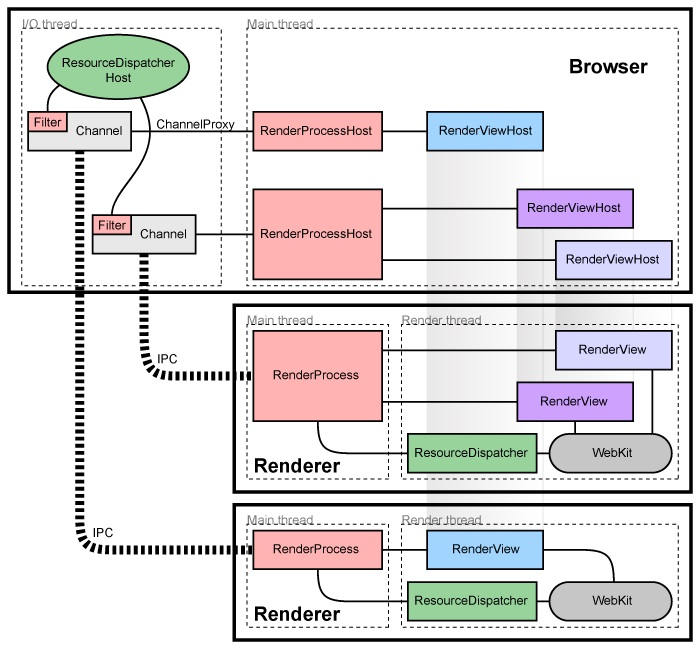
\includegraphics[scale=0.65]{figures/archGC.jpg}
        \caption{Architectura Multiprocesos de Google Chrome. Fuente: \cite{multiProcGC}}
        \label{fig:archGC}
    \end{figure}

    En la documentación de Google Chromium \cite{multiProcGC}, que es base para Google Chrome, se afirma que la arquitectura soporta para cada tab un proceso nuevo, de manera de hacer al \textit{Browser} más robusto y modularizar el sistema para evitar ciertas amenazas de seguridad; por lo que es una arquitectura Modular o Multiprocesos. El proceso principal es llamado \textit{Browser Process/Kernel/Engine} y se encarga de la Interfaz de Usuario, manejo de las tabs y los procesos de los \textit{plug-in}. Cada tab es asociado un Rendering Engine, éstos tienen restricciones de acceso (\textit{Sandboxing}) a los demas y al sistema, lo que permite que exista una protección de la memoria y un control de acceso. Google Chrome expone en \cite{reis2009browser} que existen ciertas lecciones que han ido utilizando para mejorar la calidad de su browser, éstas son:

    \begin{itemize}
    	\item Reducción de las vulnerabilidades de seguridad. Se basa en la aislación de ciertos componentes y la reducción de privilegios de ciertas tareas en el browser. La aislación lo lograron con la creación del Rendering Engine y el Browser Kernel, que tienen como objetivo proteger los datos del sistema de archivos. Si bien esto puede no entregar muchos beneficios a una aplicación web, si lo hace en el usuario del browser.
    	\item Reducir la ventana de vulnerabilidades. La actualización del browser se hace cada cierto tiempo de forma automática para así cubrir las vulnerabilidades que van apareciendo.
    	\item Reducción de la frecuencia de exposición. Google trabaja con StopBadware.org para entregar una mayor seguridad al descubrir nuevos tipos de ataques y vulnerabilidades relacionadas con el browser.
    \end{itemize}

    En \cite{barth2008security} se explica que el objetivo principal de esta arquitectura es poder mitigar ataques muy severos sin tener que sacrificar la compatibilidad con los sitios web ya existentes. Para lograr el objetivo Google ha ganado muchas lecciones de cómo realizar esto \cite{reis2009browser}, pues explican que un gran desafío en la seguridad es proteger a los usuarios de los atacantes que se aprovechan de las vulnerabilidades y debilidades de los Web Browsers. En su arquitectura modular se puede ver que se intenta proveer una seguridad que evita afectar la compatibilidad con otros sitios. La arquitectura comentada se basa en dos decisiones de diseño: La arquitectura depende en el Rendering Engine para aquellos componentes de alto riesgo como JavaScript, el parser de HTML y la creación de DOM para hacer cumplir SOP; al estar rodeados por un Sandboxing, hace que el Rendering Engine se comporte como una caja negra. 

 \subsection{Browser Kernel/Process y Renderering Engine/Process}
    El Browser Process provee al usuario con lo necesario para el manejo de sesiones (cookies, tokens, etc), historial, almacenamiento de passwords, manejo de interfaz de usuario, barra de localización, sistema local de blacklist, API para realizar llamadas al sistema tanto para almacenar datos como para realizar peticiones del usuario, agente de descarga, entro otros. El Browser Kernel tiene la tarea de ser un interceptor de las llamadas de los procesos Rendering que están en un Sandbox, revisando las políticas y qué acciones están permitidas.

    \begin{figure}[h!t]
        \centering
        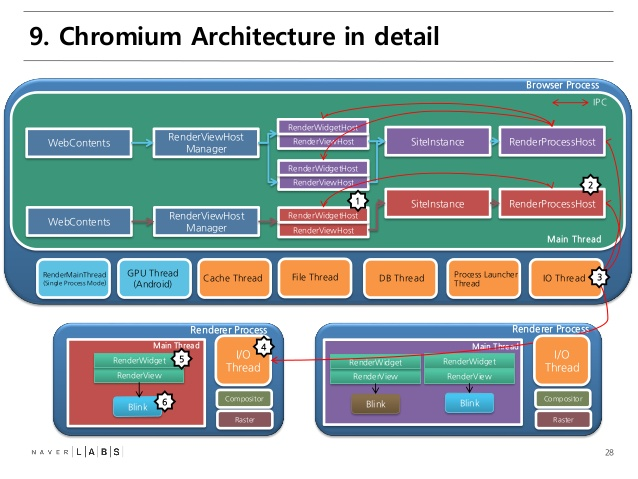
\includegraphics[scale=0.65]{figures/chromium-rendering-pipeline-28-638.jpg}
        \caption{Architectura de Chromium en detalle. Fuente: \cite{ChrRenderPipe}}
        \label{fig:archGC2}
    \end{figure}

    El \textit{Rendering Engine} usado por Google Chrome/Chromium, llamado Blink, es un \textit{forking} del trabajo original llamado Webkit. Su objetivo principal es soportar la arquitectura de multiprocesos que posee el navegador, y al mismo tiempo poder reducir el nivel de complejidad. Cada nueva ventana o tab abre un nuevo proceso, y el \textit{Browser} instruye a ese proceso a crear un componente que permitirá la visualización del recurso en el navegador. Cada proceso abierto para instanciar un Renderer estará en un Sandbox, donde puede pasar que 2 \textit{tabs} de diferentes dominios estén en el mismo proceso, dado que puede haber una relación en la navegación de estas páginas.


    %     \begin{figure}[h!t]
    %     \begin{center}
    %         \includegraphics[scale=0.5]{figures/in_process_plugins.png}
    %       %\caption{Representación conceptual de una Nube con Eucalyptus. La especificación de las partes y su explicación se ve en \ref{sec:chap2.4.2}. Fuente \cite{EucalyptusOverview}}
    %       \label{fig:archG}
    %     \end{center}
    % \end{figure}

    %\subsection{Extensions}

    %\subsection{Plugins}
    %En el ultimo tiempo, los plugins como Adobe Flash

\section{Internet Explorer}
    \label{chap3:IE}
    Internet Explorer es el navegador gráfico predeterminado por Microsoft y que su primera versión 1.0 fue realizada en 1995. IE es una derivación de Spyglass Mosaic desarrolado por la NCSA (National Center for Supercomputing Applications). En primera instancia fue un navegador que podría ser obtenido si era comprado como complemento de \textit{Microsoft Plus!} o mediante la versión \textit{OEM} de Windows 95. Desde la tercera versión de IE, en 1996, que esta se lanzó de forma gratuita.
            
    La arquitectura de este navegador es modular y permite al desarrollador utilizar los recursos para crear diferentes funcionalidades; ejemplo de esto son: toolbars, Microsoft Active X controls, etc. En la Figura \ref{fig:archIE} \cite{IEArch} se puede ver los principales componentes de la arquitectura del browser mencionado. IE utiliza \textit{COM} o \textit{Component Object Model}, una interfaz binaria estándar para componentes de software introducida por Microsoft en 1993 y que permite una comunicación entre procesos/componentes de software provenientes de la familia de software de Microsoft. \textit{COM} es similar a otras tecnologías de interfaz de componentes de software como CORBA y Java Beans. El uso de \textit{COM} gobierna la forma y la interacción de los componentes que se comunican, y permite que haya un reuso y extensibilidad de éstos.
            
	\begin{figure}[h!t]
	    \centering
		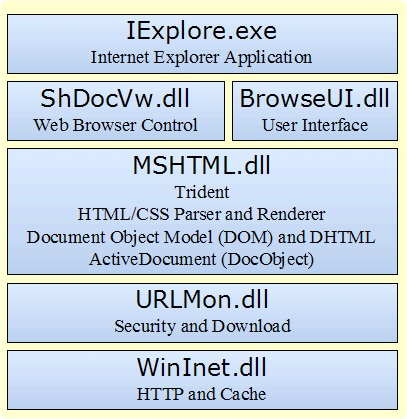
\includegraphics[scale=0.65]{figures/IEArch.jpg}
		\caption{Arquitectura de Internet Explorer. Fuente: \cite{IEArchImg}}
		\label{fig:archIE}
    \end{figure}

    \begin{figure}[h!t]
        \centering
        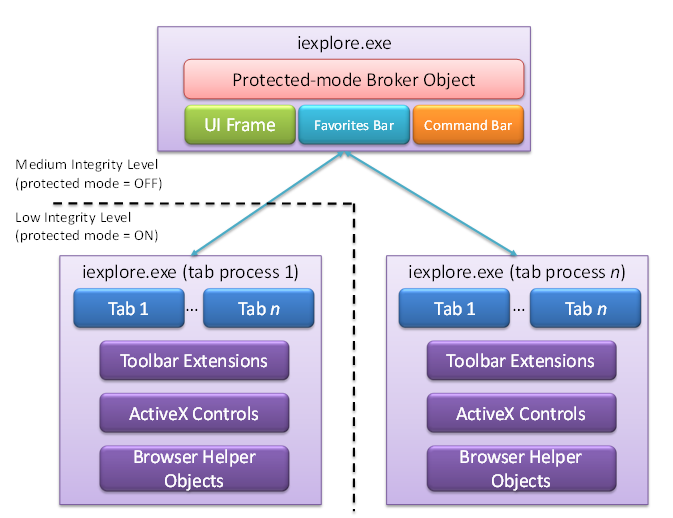
\includegraphics[scale=0.5]{figures/11_IE8andLooselyCoupledIELCIE_2.png}
        \caption{Arquitectura de Internet Explorer más detallada. Fuente: \cite{IE8LCIE}}
        \label{fig:archIE2}
    \end{figure}

    \subsection{Frame Process y Rendering Engine}   
        \label{chap2:Trident}
        MSHTML es un Rendering Engine privativo, sin embargo es posible usarlo como librería de Windows \textbf{mshtml.dll}. Según \cite{Crowley2010} es un objeto OLE (Object Linking and Embedding) Active Document que representa el \textit{layout} de Internet Explorer y permite mostrar graficamente las páginas por medio del \textit{display} del host. Dentro de éste se manejan las Extensiones, el \textit{engine} de Javascript y la librería que contiene la API para tareas de \textit{networking}, además de proveer una capa de seguridad y manejar las descargas de archivos.

    %\subsection{HBO}

    %\subsection{Plugins}


\section{Firefox}
    \label{chap3:Firefox}

    Firefox fue creado en 1998 a partir del navegador \textit{Netscape}. Actualmente la fundación Mozilla ha sido la que la ha mantenido, generando varias modificaciones desde su nacimiento. Las metas de diseño que Mozilla desee en el navegador son:
    \begin{itemize}
        \item Renderizado rápido de las páginas web.
        \item Fuerte apoyo a los estándares web como la W3C.
        \item Interoperabilidad en las diversas plataformas.
    \end{itemize}

    \subsection{Firefox Monoproceso y Gecko}
        \begin{figure}[h!t]
    		\centering
        	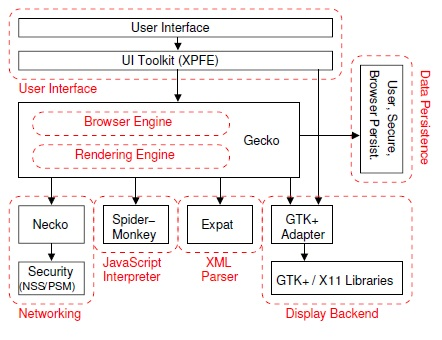
\includegraphics[scale=0.85]{figures/archMoz.jpg}
            \caption{Arquitectura Monoproceso obtenida en Fuente \cite{2005-grosskurth-browser-refarch, preprint-grosskurth-browser-archevol}}
            \label{fig:archM}
        \end{figure}
                
        La arquitectura de este browser puede ser vista en la Figura \ref{fig:archM}, donde se pueden observar los siguientes componentes principales:
                \begin{itemize}
                    \item La interfaz de usuario, la cual puede ser reutilizada para otras aplicaciones por su bajo acoplamiento con el sistema entero. 
                    \item La persistencia de los datos, tanto de bookmarks como de datos de bajo nivel como el \textit{cache}.
                    \item EL \textit{Rendering Engine}, que permite el renderizado de documentos HTML/XML por un tipo de parser basado en web estándars. Este Engine es capaz de renderizar la interfaz de la aplicación multiplataforma.
                    \item XPCOM o Cross Platform Component Object Model, similar a Microsoft COM, proporciona un conjunto básico de componentes que pueden ser implementados en diferentes lenguajes.
                \end{itemize}
        La arquitectura de Mozilla se distingue de las demás en que la visualización especificada por la plataforma y la librería de \textit{widgets} son usados directamente en el navegador, lo que minimiza el costo necesario para soportar diferentes plataformas. Si bien esta figura muestra lo más importante, algunos detalles relevantes son olvidados, como las extensiones y el componente XPCOM (cross, platform component object model) que es similiar al componente COM de Microsoft,

        Gecko es un motor de renderizado \textit{Open Source} que utiliza Firefox, escrito en C++, creado en un comienzo por Netscape, predecesor de Mozilla Foundation/Corporation. La función de este componente en Firefox (y otros browsers que lo integran) es leer el \textit{web content} de tipo HTML, CSS, XUL (para renderizar Interfaz de Usuario) y Javascript, y mostrarlo al usuario en un formato gráfico. Tiene un gran rendiemiento al transformar a formato gráfico una página con lenguaje de marcado, ya que soporta multithreading en el parser de HTML. Gecko fue diseñado para soportar \textit{Open Internet Standards}, y por ende sigue al pie de la letra todas las especificaciones de HTML 4, CCS 1 y 2, DOM, XML y Javascript. Los componentes de Gecko incluyen:
            \begin{itemize}
                \item Parser de Documentos (HTML y XML).
                \item \textit{Layout Engine} con un modelo de contenido; ésta es la información que el display del host mostrará al usuario.
                \item Sistema de estilos.
                \item Motor de Javascript. En el caso de Gecko éste se llama \textbf{SpiderMonkey} que está escrito en C/C++.
                \item Librería de imágenes.
                \item Librería de \textit{Networking} o Necko.
                \item Renderizado gráfico específico a la plataforma y widget de acuerdo al sistema operativo.
                \item Librerías de seguridad, NSS
                \item Mozilla Plug-in API (NPAPI).
                \item Lbrería de preferencias de usuario, entre otros más.

            \end{itemize}
        En la figura \ref{fig:Gecko} se explica como el Rendering Engine es capaz de crear una página a través de un HTML y su correspondientes CSS. Éste parte como 2 pipelines que leen tanto HTML como CSS, y cuando llegan al Frame Constructor, se vuelven una. Ya en esa fase, se espera que solo una hebra se encargue del contenido visual que se mostrará, pues si se tuviera más habría problemas con las prioridades de los elementos a mostrar en el DOM y el Layout final.

        Finalmente, en el día de hoy los Plugins ya son considerados tecnología \textit{legacy}, en especial el uso de Adoble Flash, que estaba bien arraigado. Ahora se ha empezado a utilizar HTML5 como una alternativa que se ajusta a los estándares de la W3C.

        \begin{figure}[h!t]
            \centering
            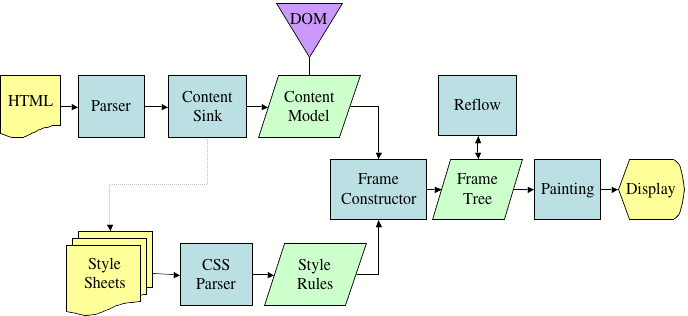
\includegraphics[width=0.85\textwidth]{figures/Gecko_Overview_9.png}
            \caption{Gecko Rendering Engine. Fuente: \cite{gecko}}
            \label{fig:Gecko}
        \end{figure}

        \subsubsection{Estabilidad y Recuperación a fallos}
        Este tipo de Firefox utiliza un proceso que se encarga de realizar tanto el Renderizado como la comunicación con las páginas web, y tiene la desventaja de que si sufre un fallo pequeño, todas las Tabs asociadas al proceso pueden ser corrompidas por el fallo. Así como también, el cierre inesperado puede causar una pérdida total de los datos. Aunque Firefox sea uno de los \textit{Browser} con mejor compatibilidad y sigue bastante bien los estandares Web de la W3C, le ha sido bastante difícil moverse a una arquitectura Modular como Google Chrome y Explorer \cite{ElectrolysisTalk}
        
    \subsection{Firefox Multiproceso (Electrolysis, e10s)} 
    El proyecto Electrolysis o e10s, comenzó el 2009 y que por motivos desconocidos \cite{ElectrolysisTalk} se tuvo que poner en espera. El 2012 la Arquitectura del Sistema Operativo Firefox empezó a usar la idea de multiprocesos que se había estado trabajando, por lo que el 2013 se recontinuó el proyecto, sin embargo aún no hay una versión estable y solo se puede ocupar como testing en la versión Nightly Build \cite{NightlyBuilds}. La nueva Arquitectura se basa en usar la aislación que provee el sistema operativo a los procesos, de la misma manera que lo hace Google Chrome, pero por supuesto el diseño no es el mismo.

    \subsubsection{Chrome Process y Content Process}
    Respecto a este componente de la nueva arquitectura que Electrolysis, no mucha información de que es lo que hace está en línea. Parte de los componentes son el sistema de comunicación que existe entre los procesos o Message Manager, que se encarga de enviar mensajes de control desde el Chrome Process a los procesos hijos o recibir los mensajes desde sus procesos hijos para realizar las acciones necesarias para mostrar el contenido (Figura \ref{fig:ChromePComm1}, \ref{fig:ChromePComm2}).
        \begin{figure}[h!t]
            \centering
            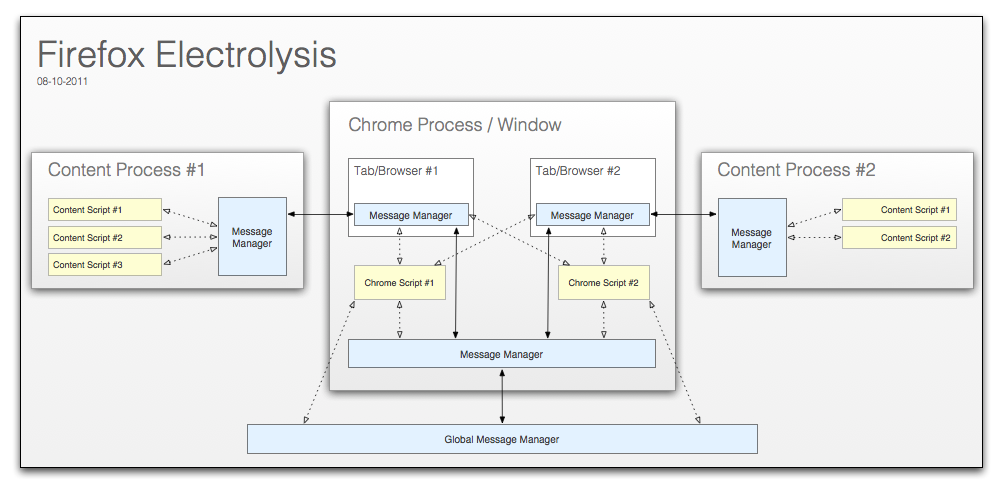
\includegraphics[width=1\textwidth]{figures/electrolysis.png}
            \caption{Firefox Electrolysis, Comunicación de procesos 1. Fuente: \cite{Firefox101}}
            \label{fig:ChromePComm1}
        \end{figure}

    Así como Google e Internet Explorer, se tiene en Electrolysis al Chrome Process como intermediario para cualquier tipo de acción dentro del \textit{Browser} lo que permite controlar las peticiones del usuario o scripts que se ejecuten en el Content Process (hijo). Finalmente, la propuesta que han desarrollado con Electrolysis, si bien ha capturado buenas prácticas, aún no ha podido realizar una implementación del Sandbox y está lejos aún.

        \begin{figure}[h!t]
            \centering
            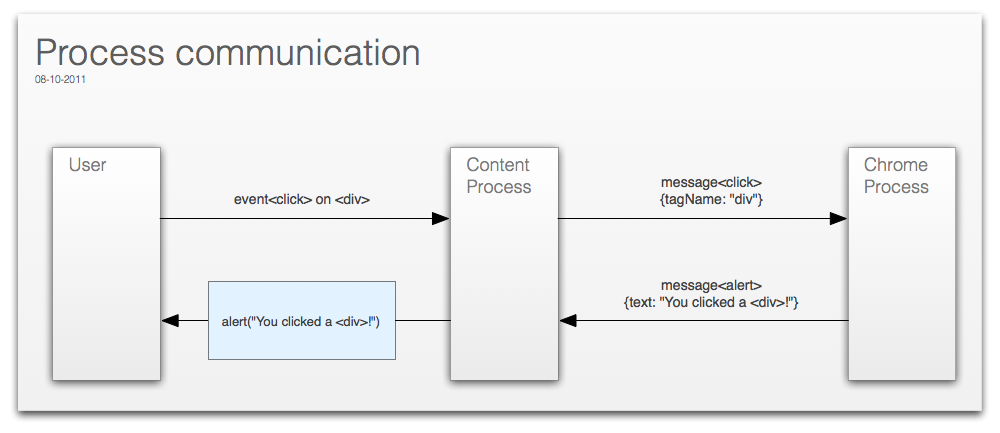
\includegraphics[width=1\textwidth]{figures/e10s-processes.png}
            \caption{Firefox Electrolysis, Comunicación de procesos 2. Fuente: \cite{Firefox101}}
            \label{fig:ChromePComm2}
        \end{figure}

    


% \subsection{Rendering Engines}
% \label{chap2:RenderingE}
% Responsable de converitir la página web, en HTML o XML, a un formato visible cómodo para el usuario en la pantalla del host. La combinación de HTML, CSS y media (imagenes, videos, etc.) permiten entregar una experiencia gráfica al usuario con la que interactuará. Existen browser que no usan gráficos y solo se basan en mostrar texto, ejemplos de estos navegadores son: W3M y Lynx. Los \textit{Rendering Engines} más usados son: Webkit (Safari), Blink (Google Chrome/Chromium), Trident (Internet Explorer) y Gecko (Firefox).

%     \subsubsection{Trident}
%     
%     







